\section{Ogólne określenie wymagań}		%1
%Ogólne określenie wymagań i zakresu programu (Czyli zleceniodawca określa wymagania programu) 

\hspace{0.60cm}Nowoczesne smartfony są naszpikowane różnego rodzaju czujnikami. To one sprawiają, że codzienne używanie telefonów komórkowych jest łatwe i przyjemne. Dzięki nim urządzenia znają naszą lokalizacji, w którym kierunku się poruszamy oraz sposób w jaki je trzymamy. Wygaszanie ekranu, gdy zbliżymy słuchawkę do policzka, automatyczna zmiana orientacji wyświetlanego obrazu, kiedy obrócimy telefon czy
w końcu sterowanie zaawansowanymi grami - to wszystko nie byłoby możliwe bez czujników. Ogólnym zamysłem naszego projektu jest stworzenie aplikacji która ma służyć do testowania czujników w telefonach, co ułatwiłoby i bardzo przyśpieszyło pracę w naszym serwisie komórkowym. \newline 

Zależy nam na możliwości sprawdzenia czujników takich jak: \\
- latarka, \\
- czujnik zbliżeniowy, \\
- gps, \\
- wifi, \\
- dźwięk, \\
- mikrofon, \\
- aparat.\\

\begin{figure}[!hbt]
	\begin{center}
		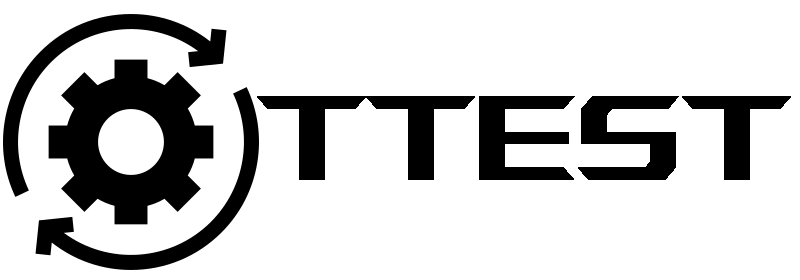
\includegraphics[angle=360, width=0.65\textwidth]{rys/punkt1/logo_black.png}
		\caption{Logo firmy TTest}
		\label{rys:logo}
	\end{center}
\end{figure}

Nasza firma powstała w 2011 roku; przez ponad 10 lat prężnie pracujemy oraz staramy się zadbać nie tylko o naszych klientów lecz i o naszych pracowników, stąd też pojawił się pomysł na wdrożenie nowej aplikacji, która pozoliłaby na jeszcze wiekszę usprawnienie pracy w naszym zespole. Co roku przybywa nam tysiące nowych klientów którzy liczą na fachową pomoc z naszej strony, z związku z tym zatrudniamy coraz więcej nowych pracowników i to właśnie do nich w dużej mierze miałaby trafić nowa aplikacja testująca. 

\newpage

Nasza firma posiadała w przeszłości już jedną aplikacje, niestety przez upływ czasu stała się przestarzała i nie spełnia naszych obecnych wymagań, np. brak testu lokalizacji, który obecnie jest jednym z podstawowych czujników wykorzystywanym w wielu aplikacjach. Co więcej wygląd aplikacji jest przestarzały na obecne standardy, test trzeba było wybrać z rozwijanej listy, która stała się niepraktyczna oraz mocno spowalniała pracę, dlatego zależy nam aby layout nowej aplikacji był zachowany w intuicyjny i minimalistyczny sposób, przez co nawet osoby które dopiero odbywają szkolenia w naszej firmie mogły wspomóc pracowników i same przeprowadzać testy poszczególnych czujników. Również zależy nam aby w aplikacji można było w jakiś sposób podsumować przeprowadzone testy. Kolorem przewodnim naszej firmy jest niebieski, dlatego zależy nam na tym aby akcenty właśnie w tym kolorze pojawiły się w aplikacji; mogą to być na przykład przyciski czy chociażby kolor tła aplikacji. Na rysunku \ref{rys:logo} znajduję się logo naszej firmy, zależy nam aby pojawiło się jako ikonka aplikacji oraz w samej aplikacji. \newline 

Myślimy o prostej i przejrzystej budownie menu, składajacych się z dużych kafelków które będą odnośnikiem do poszczególnych testów. Zobrazowanie naszego pomysłu znajduje się na rysunku \ref{rys:layout}. \newline

Jeśli chodzi o przyciski to zależałoby nam na tym aby pojawiły się ikonki przedstawiające daną funkcje, na przykład zamiast samego napisu "Latarka" pojawił się przycisk z wizerunkiem przedstawiającym latarke, co sprawi to że aplikacja będzie wyglądać przejrzyście i w szybki sposób będzie można wzrokowo znaleść interesujący nas test. 

\begin{figure}[!hbt]
	\begin{center}
		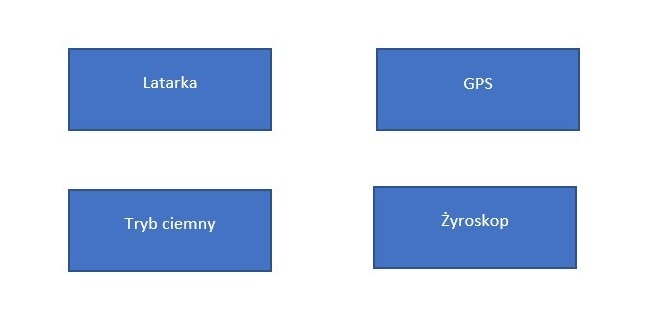
\includegraphics[angle=360, width=0.80\textwidth]{rys/punkt1/Layout_1.jpg}
		\caption{Przykładowy layout}
		\label{rys:layout}
	\end{center}
\end{figure}





  


 
 
 
 
 